\section{Leading-Zero-Counter and Shifter (LZCS) Compilation Example}
\label{sec:lzc}
In this section we provide an LZCS DFiant implementation and describe its compilation process. We begin with a pseudo code reference implementation\cite{muller2009handbook} as depicted in \fig{fig:LZC_pseudo_code}. The DFiant LZCS implementation\footnote{This code was also utilized to implement FPMul in DFiant} is very similar to the pseudo code reference, as can be seen in \fig{fig:LZC_DFiant_code}.
\begin{figure}[h]
\begin{algorithm}[H]
  \caption*{Combined leading-zero counting and shifting}
  \begin{algorithmic}
    \small
    \STATE{$k \leftarrow \left\lceil \log_2{n} \right\rceil$}
    \STATE{$x_k \leftarrow x$}
    
    \FOR{$i = k-1$ downto $0$}
    \IF{there are $2^i$ leading zeros in $x_{i+1}$} 
    \STATE{$d_i \leftarrow 1$}
    \STATE{$x_i \leftarrow x_{i+1}$, shifted left by $2^i$}
    \ELSE 
    \STATE{$d_i \leftarrow 0$}
    \STATE{$x_i \leftarrow x_{i+1}$}
    \ENDIF
    \ENDFOR
    \STATE{return $(d, x0)$}
  \end{algorithmic}
\end{algorithm}
\captionof{figure}{LZCS pseudo code reference}
\label{fig:LZC_pseudo_code}
\end{figure}

\begin{figure}[h]
  \begin{minted}[autogobble,tabsize=2,frame=single,fontsize=\small]{Scala}
    def lzcs[N](num : DFBits[N]) = {
      val k = log2Up(num.width)
      val x = DFBits(num.width) := num
      val d = DFBits(k) := 0
      
      for (i <- k-1 downto 0) {
        ifdf (x.msbits(2~^i) == 0) {
          d(i) := 1
          x := x << 2~^i
        }
      }
      (d, x)
    }
  \end{minted}
  \captionof{figure}{LZCS DFiant code}
  \label{fig:LZC_DFiant_code}
\end{figure}

When we apply \code{lzcs} on an 8-bit vector \code{num}, the DFiant frontend compiler unrolls the \code{for} loop and converts the \code{ifdf} control statements into multiplexer nodes. An equivalent unrolled code is given in \fig{fig:LZC_unrolled_code}. This code is similar to the frontend compiler's static single assignment (SSA) intermediate representation (IR) form. The DFiant frontend IR is a dataflow dependency graph as illustrated in \fig{fig:LZC_Dataflow}. We can optimize the IR design independently of the target device. For example, we can derive \code{d\_i} directly from \code{c\_i} and remove unnecessary multiplexer nodes.

\begin{figure}[h]
  \begin{minted}[autogobble,tabsize=2,frame=single,fontsize=\small]{Scala}
	val x_3 = DFBits[8] := num;	 val d_3 = DFBits[3] := 0
	val c_2 = x_3(7,4)==0;        val X_3 = x_3 << 4
	val x_2 = mux(c_2, X_3, x_3); val D_3 = d_3(2):=1
	val d_2 = mux(c_2, D_3, d_3)
	val c_1 = x_2(7,6)==0;        val X_2 = x_2 << 2
	val x_1 = mux(c_1, X_2, x_2); val D_2 = d_2(1):=1
	val d_1 = mux(c_1, D_2, d_2)
	val c_0 = x_1(7,7)==0;        val X_1 = x_1 << 1
	val x_0 = mux(c_0, X_1, x_1); val D_1 = d_1(0):=1
	val d_0 = mux(c_0, D_1, d_1)
	return (d_0, x_0)
  \end{minted}
  \captionof{figure}{LZCS unrolled code for an 8-bit input}
  \label{fig:LZC_unrolled_code}
\end{figure}

The backend compiler converts the dataflow graph to Verilog and adds pipeline registers as required to achieve the target performance.
Not all dataflow nodes cost logic and therefore do not affect performance. Bit referencing, concatenation, shifting, and assignment do not cost any hardware resources (software backend compilation can incur performance  penalty). 

The preliminary auto-pipelining backend compiler we implemented relies on an estimation database that is used to calculate each node's potential propagation delay cost. The compiler makes sure no path propagation delay surpasses the target clock period, including a fixed safe margin for additional wiring delay that may occur during placement and routing. Strategic register placement brakes down long paths but increases the path clock cycle latency. All converging paths must possess the same latency to maintain correctness (we can rely on token exchange signals to provide dependency correctness, but to achieve optimal performance we need to balance the paths' latency nonetheless).

\begin{figure}[h]
  \centering
  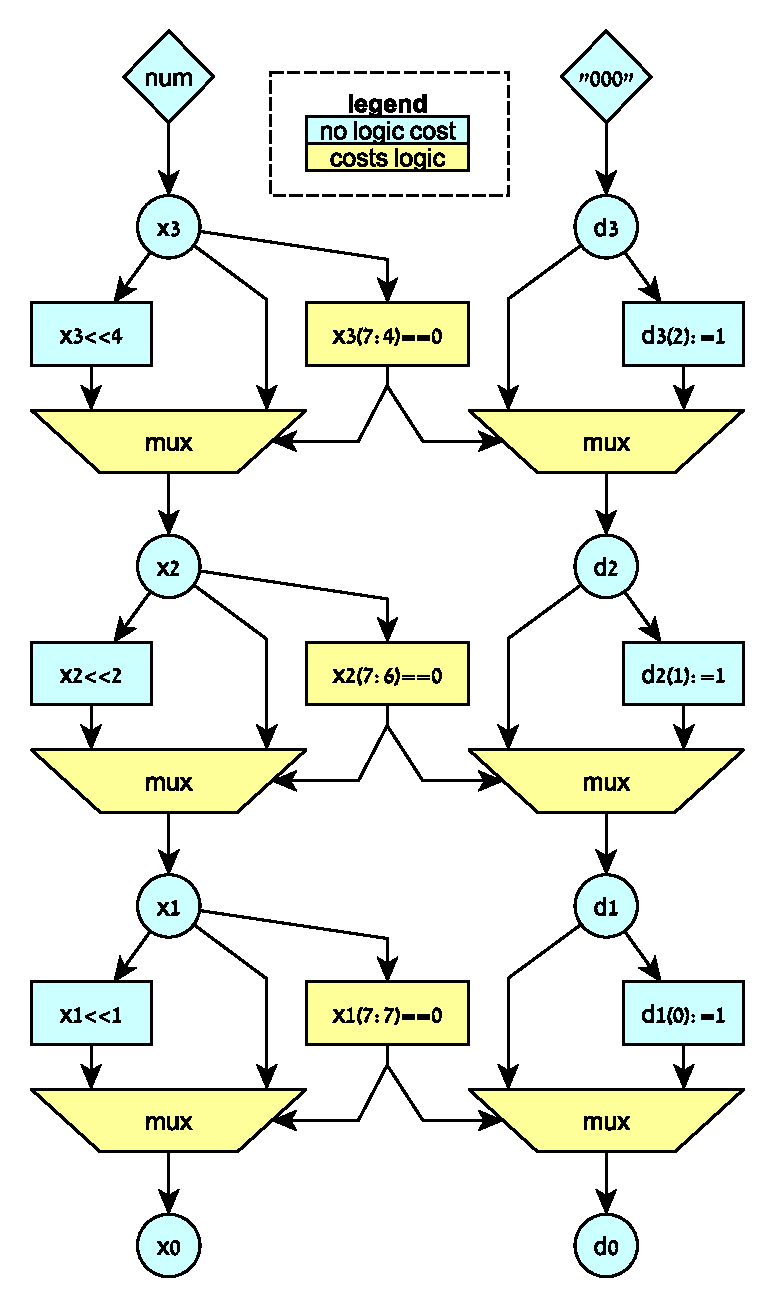
\includegraphics[width=0.8\linewidth]{graphics/lzc_dataflow.pdf}
  \captionof{figure}{LZCS IR graph for an 8-bit input}
  \label{fig:LZC_Dataflow}
\end{figure}
